\documentclass[aspectratio=169]{beamer}
%\documentclass[aspectratio=169,handout]{beamer}
\usepackage[utf8]{inputenx} % For æ, ø, å
\usepackage{csquotes}       % Quotation marks
\usepackage{microtype}      % Improved typography
\usepackage{amssymb}        % Mathematical symbols
\usepackage{mathtools}      % Mathematical symbols
\usepackage[absolute, overlay]{textpos} % Arbitrary placement
\setlength{\TPHorizModule}{\paperwidth} % Textpos units
\setlength{\TPVertModule}{\paperheight} % Textpos units
\usepackage{tikz}
\usetikzlibrary{overlay-beamer-styles}  % Overlay effects for TikZ


\AtBeginSection{\frame{\sectionpage}}
\AtBeginSubsection{\frame{\subsectionpage}}

\usepackage{hyperref}
\usepackage{svg}
%\usefonttheme{serif}

\usepackage{xfrac}
\usepackage{soul} % Colored text and highlighting, respectively
\usepackage{xcolor}
\usepackage{tikz-cd} % For commutative diagrams
\usepackage{tikz-3dplot}
\usetikzlibrary{angles}
\RequirePackage{pgfplots}
\usepackage{mathtools}
\usepackage{answers}
\usepackage{setspace}
\usepackage{graphicx}
\usepackage{enumerate}
\usepackage{multicol}
%\usepackage{mathrsfs}
\usepackage{amsmath,amsthm}
\usepackage{marvosym,wasysym} %fucking smileys
\usepackage{float}
\usepackage{morefloats}
\usepackage{pgf,tikz}
\pgfplotsset{compat=1.15}
%\usepackage{mathrsfs}
\usetikzlibrary{arrows}
\usepackage{subcaption}
\usepackage[most]{tcolorbox}
\tcbuselibrary{theorems}
\usepackage{fancyvrb}
\usepackage{longtable,booktabs}
\usepackage{stackrel}
\usepackage{animate}
\usepackage[percent]{overpic}
\definecolor{lighter_csu_green}{RGB}{60,133,77}
\definecolor{csu_gold}{RGB}{198,184,77}
\definecolor{gray}{RGB}{60,60,60}
\newcommand\boldgreen[1]{\textcolor{lighter_csu_green}{\emph{\textbf{#1}}}}
\newcommand\boldgold[1]{\textcolor{csu_gold}{\textbf{#1}}}
\usepackage{MnSymbol}
%border matrix
\makeatletter
\newif\if@borderstar
\def\bordermatrix{\@ifnextchar*{%
\@borderstartrue\@bordermatrix@i}{\@borderstarfalse\@bordermatrix@i*}%
}
\def\@bordermatrix@i*{\@ifnextchar[{\@bordermatrix@ii}{\@bordermatrix@ii[()]}}
\def\@bordermatrix@ii[#1]#2{%
\begingroup
\m@th\@tempdima8.75\p@\setbox\z@\vbox{%
\def\cr{\crcr\noalign{\kern 2\p@\global\let\cr\endline }}%
\ialign {$##$\hfil\kern 2\p@\kern\@tempdima & \thinspace %
\hfil $##$\hfil && \quad\hfil $##$\hfil\crcr\omit\strut %
\hfil\crcr\noalign{\kern -\baselineskip}#2\crcr\omit %
\strut\cr}}%
\setbox\tw@\vbox{\unvcopy\z@\global\setbox\@ne\lastbox}%
\setbox\tw@\hbox{\unhbox\@ne\unskip\global\setbox\@ne\lastbox}%
\setbox\tw@\hbox{%
$\kern\wd\@ne\kern -\@tempdima\left\@firstoftwo#1%
\if@borderstar\kern2pt\else\kern -\wd\@ne\fi%
\global\setbox\@ne\vbox{\box\@ne\if@borderstar\else\kern 2\p@\fi}%
\vcenter{\if@borderstar\else\kern -\ht\@ne\fi%
\unvbox\z@\kern-\if@borderstar2\fi\baselineskip}%
\if@borderstar\kern-2\@tempdima\kern2\p@\else\,\fi\right\@secondoftwo#1 $%
}\null \;\vbox{\kern\ht\@ne\box\tw@}%
\endgroup
}
\makeatother

\usetheme{UiB}

%For easier reading
\setbeamersize{text margin left=40pt,text margin right=40pt}
\renewcommand{\baselinestretch}{1.3}


%% FONT STUFF
\usefonttheme[onlymath]{serif}

%Commands
\newcommand{\R}{\mathbb{R}}
\newcommand{\C}{\mathbb{C}}
\newcommand{\opens}{\mathcal{O}}
\newcommand{\hilbert}{\mathcal{H}}
\newcommand{\algebra}{\mathcal{A}}
\newcommand{\ideals}{\mathcal{I}}
\newcommand{\functionals}{\mathcal{M}}
\newcommand{\spec}{\mathrm{spec}}
\newcommand{\clifford}{\mathrm{C}\ell}
    \newcommand\quotient[2]{
        \mathchoice
            {% \displaystyle
                \text{\raise1ex\hbox{$#1$}\Big/\lower1ex\hbox{$#2$}}%
            }
            {% \textstyle
                #1\,/\,#2
            }
            {% \scriptstyle
                #1\,/\,#2
            }
            {% \scriptscriptstyle  
                #1\,/\,#2
            }
    }

% Special Commands
\newcommand{\bigslant}[2]{{\raisebox{.2em}{$#1$}\left/\raisebox{-.2em}{$#2$}\right.}}
\newcommand{\RE}{\mathrm{Re}}
\newcommand{\IM}{\mathrm{Im}}
\newcommand{\multivectorbundle}{\mathcal{G}(M,g)}
\newcommand{\multivectorfields}{\mathcal{G}(M)}
\newcommand{\differentialforms}{\mathcal{G}^*(M)}
\newcommand{\kvectorfields}[1]{\mathcal{G}^{#1}(M)}
\newcommand{\evenfields}{\mathcal{G}^{[0]}(M)}
\newcommand{\oddfields}{\mathcal{G}^{[1]}(M)}
\newcommand{\id}{\mathrm{id}}
\newcommand{\innerproduct}[2]{\left\langle #1, #2 \right\rangle_{L_2(\Sigma)}}
%\newcommand{\algebra}[1]{\mathcal{A}_{#1}}
\newcommand{\grad}{\boldsymbol{\nabla}}
\newcommand{\dirac}{\boldsymbol{D}}
\newcommand{\geometricalg}{\mathcal{G}(V)}
\newcommand{\spacealg}{\mathcal{G}_3}
\newcommand{\dual}[1]{\overset{$\star$}&{#1}}
\newcommand{\G}{\mathcal{G}}
\newcommand{\cauchy}{\mathcal{C}}
\newcommand{\poisson}{\mathcal{P}}
\newcommand{\tangent}{\boldsymbol{t}}

\newcommand{\openO}{\mathcal{O}}
\newcommand{\openU}{\mathcal{U}}
\newcommand{\characters}{\mathfrak{M}}
\newcommand{\Span}{\operatorname{Span}}
\newcommand{\paravectors}{\mathcal{P}}
\newcommand{\paravectorfields}{\mathcal{P}(M)}
\newcommand{\monogenics}{\mathcal{M}}
\newcommand{\dualmonogenics}{\mathcal{M}^*}
\newcommand{\Grassmannian}[2]{\textrm{Gr}(#1,#2)}
\newcommand{\spinalgebra}{\mathfrak{spin}(n)}
\newcommand{\spingroup}{\operatorname{Spin}(n)}
\newcommand{\ball}{\mathbb{B}}
\newcommand{\disk}{\mathbb{D}}
\newcommand{\projection}{\operatorname{P}}
\newcommand{\vectorspace}{\mathbb{V}}
\newcommand{\multivectorfieldson}[1]{\mathcal{G}(#1)}
\newcommand{\biparavectorfieldson}[1]{\mathcal{G}_n(#1)^{0+2}}
\newcommand{\spinnorm}[1]{\|#1\|_{L_2}}
\newcommand{\rejection}{\operatorname{R}}
\newcommand{\vectorpotential}{\mathbf{A}}
\newcommand{\current}{\blade{j}}
\newcommand{\magneticbivector}{\blade{b}}
\newcommand{\cross}{\boldsymbol{\times}}
\newcommand{\blade}[1]{\boldsymbol{#1}}
\newcommand{\intcurrent}[1]{\left[ #1 \right]}
\newcommand{\multivecinnerproduct}[2]{\ll #1, #2\gg}
\newcommand{\spacetime}{\boldsymbol{\gamma}}
\newcommand{\gradst}{\boldsymbol{\nabla}_{\textrm{ST}}}
\newcommand{\boundary}{{\partial M}}
\newcommand{\normalcurrent}{\blade{j}^{\blade{\nu}}}
\newcommand{\tangentialcurrent}{\blade{j}^{\blade{I}_\partial}}
\newcommand{\normal}{\blade{\nu}}
\newcommand{\pseudoscalar}{\blade{I}}

\newcommand{\kforminnerproduct}[2]{\llangle #1, #2 \rrangle}

\DeclarePairedDelimiter\angles{\langle}{\rangle}
\newcommand{\proj}[2]{\angles*{#2}_{#1}}

% Forms stuff
\newcommand{\harmonicfields}[1]{\mathcal{H}^{#1}(M)}
\newcommand{\monogenicex}[1]{\mathcal{M}^{#1}_{\textrm{ex}}(M)}
\newcommand{\monogenicco}[1]{\mathcal{M}^{#1}_{\textrm{co}}(M)}
\newcommand{\monogenicdirichlet}[1]{\mathcal{M}^{#1}_D(M)}
\newcommand{\monogenicneumann}[1]{\mathcal{M}^{#1}_N(M)}
\newcommand{\exactfields}[1]{\mathcal{E}^{#1}(M)}
\newcommand{\coexactfields}[1]{\mathcal{C}^{#1}(M)}
\newcommand{\monogenicfields}[1]{\mathcal{M}^{#1}(M)}
\newcommand{\cliffordoplus}{\stackrel{C\ell}{\oplus}}
\newcommand{\bivector}{\blade{B}}

\author{Colin Roberts}
\setbeamercolor{title}{fg=white} 
\title{The story of Fourier and his theory of heat and trigonometric series}
\setbeamercolor{subtitle}{fg=white} 
\subtitle{}

\setcounter{tocdepth}{1}

\usepackage[super]{nth}

\begin{document}

\begin{frame}{Overview}
\tableofcontents
\end{frame}

\section{Fourier's life}

\begin{frame}{Beginning}
\vfill
\begin{itemize}
    \pause
    \item Jean-Baptiste Joseph Fourier was born on March \nth{21}, 1768, as the son of a tailor.
    \pause
    \item He was one of twelve children and was orphaned at age 10.
    \pause
    \item He first received education at a local convent and moved to the \'{E}cole Royale Militaire of Auxerre after recommendation.
\end{itemize}
\vfill
\end{frame}

\begin{frame}{French revolution}
\vfill
\begin{itemize}
    \pause
    \item Fourier was sympathetic to the revolution since he dreamt ``of establishing among us a free government exempt from kings and priests."
    \pause
    \item He joined a local revolutionary committee.
    \pause
    \item In July 1794, His stance lead to his imprisonment and he was set to face the guillotine.
    \pause
    \item He was pardoned after the death of Maximilien Robespierre.
\end{itemize}
\vfill
\end{frame}

\begin{frame}{Education}
\vfill
\begin{itemize}
    \pause
    \item Fourier was asked to join Joseph-Louis Lagrange, Pierre-Simon Laplace, and Gaspard Monge in 1795 at the \'Ecole Polytechnique to help rebuild France.
    \pause
    \item A few years later, Fourier joined Napoleon's army as a scientific advisor for the invasion of Egypt. 
    \pause
    \item Fourier continued to teach until 1801 when Napoleon appointed him as prefect in Grenoble.
\end{itemize}
\vfill
\end{frame}

\section{The propagation of heat in solid bodies}

\begin{frame}{}
\vfill
\begin{figure}[H]
    \centering
    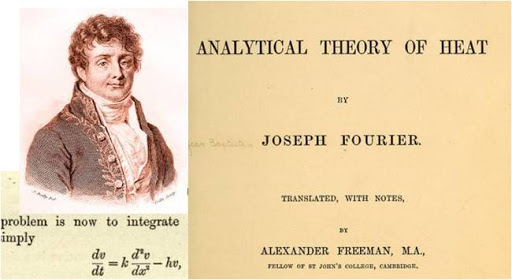
\includegraphics[width=.8\textwidth]{figures/theory_of_heat.jpg}
\end{figure}
\vfill
\end{frame}

\begin{frame}{Idea}
\vfill
    \begin{itemize}
        \pause
        \item No one knew the mechanism of heat flow during Fourier's time.
        \pause
        \item Fourier assumed that heat moved linearly through a medium.
    \end{itemize}
\vfill
\end{frame}

  \begin{frame}{Conduction}
\vfill
\begin{columns}
\begin{column}{0.5\textwidth}
   \vfill
    \begin{itemize}
        \item Let $T_1$ and $T_2$ be temperatures of two slabs.
        \item Heat moves through the slabs via
        \[
        \dot{Q}= k A \frac{T_1 - T_2}{L}.
        \]
        \item In the infinitesimal case, 
        \[
        \dot{Q}=-kA \frac{dT}{dx}
        \]
    \end{itemize}
    \vfill
\end{column}
\begin{column}{0.5\textwidth}  %%<--- here
    \begin{center}
     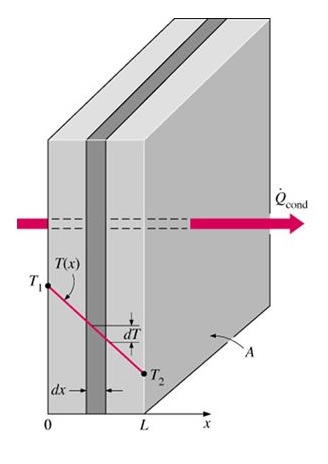
\includegraphics[width=0.5\textwidth]{figures/fourier_conduction.jpg}
     \end{center}
\end{column}
\end{columns}
\vfill
\end{frame}

\begin{frame}{Heat equation}
\vfill
\begin{itemize}
    \pause
    \item Fourier reasoned that the following must describe the rate 
    \[
    \textrm{energy in} - \textrm{energy out} + \textrm{energy generated} = \textrm{accumulated energy}.
    \]
    \vspace*{-.30cm}
    \pause
    \item Fourier used dimensional analysis to reveal that
    \[
    (\dot{Q}(x+\Delta x)-\dot{Q}(x))A-\dot{q}A\Delta x = \rho c \frac{\partial T}{\partial t}A \Delta x.
    \]
    \vspace*{-.30cm}
    \pause
    \item In the infinitesimal case we get the heat equation
    \[
    \rho c \frac{\partial T}{\partial t} = \frac{\partial}{\partial x} \left(k \frac{\partial T}{\partial x}\right) + \dot{q}.
    \]
\end{itemize}
\vfill
\end{frame}

\begin{frame}{Heat equation}
\vfill
\begin{itemize}
    \pause
    \item Fourier also derived the equation in 3-dimensions as well!
    \pause
    \item He described the dimensions and meaning of all the constants above
    \begin{align*}
    k&= \textrm{conductivity}\\
    c&= \textrm{heat capacity}\\
    \rho&= \textrm{density}
    \end{align*}
\end{itemize}
\vfill
\end{frame}

\section{Fourier series}

\begin{frame}{Heat equation on a ring}
\vfill
\begin{itemize}
    \pause
    \item Amongst other examples, he considered heat flow on a ring.
    \pause
    \item He found a set of solutions as $e^{-n^2 \pi^2 t}\cos(2\pi n x)$ and $e^{-n^2 \pi^2 t}\sin(2\pi n x)$.
    \pause
    \item He questioned whether any initial condition could be written using these solutions.
\end{itemize}
\vfill
\end{frame}

\begin{frame}{Trigonometric series}
\vfill
\begin{itemize}
    \pause
    \item He attempts to solve
    \[
          1= \sum_{n \textrm{ odd}} a_{n} \cos(nx)
    \]
    for which he found
    \begin{align*}
    a_1 = \frac{3^2}{3^2-1^2}\cdot \frac{5^2}{5^2-1^2} \cdots \qquad a_3 = \frac{1^2}{1^2-3^2}\cdot \frac{5^2}{5^2-3^2} \cdots \dots
    \end{align*}
    and so on, then used Wallis' formula to show
    \[
    a_n = (-1)^n \frac{4}{n\pi}
    \]
\end{itemize}
\vfill
\end{frame}

\begin{frame}{}
\vfill
Eventually, he realizes
\[
\sum_{n \textrm{ odd}} (-1)^n \frac{4}{n\pi} \cos(nx) = \begin{cases} \frac{\pi}{4} & 0<x<\frac{\pi}{2} \\
    -\frac{\pi}{4} & \frac{\pi}{2}<x<\frac{3\pi}{2}\end{cases}
\]
\begin{figure}[H]
    \centering
    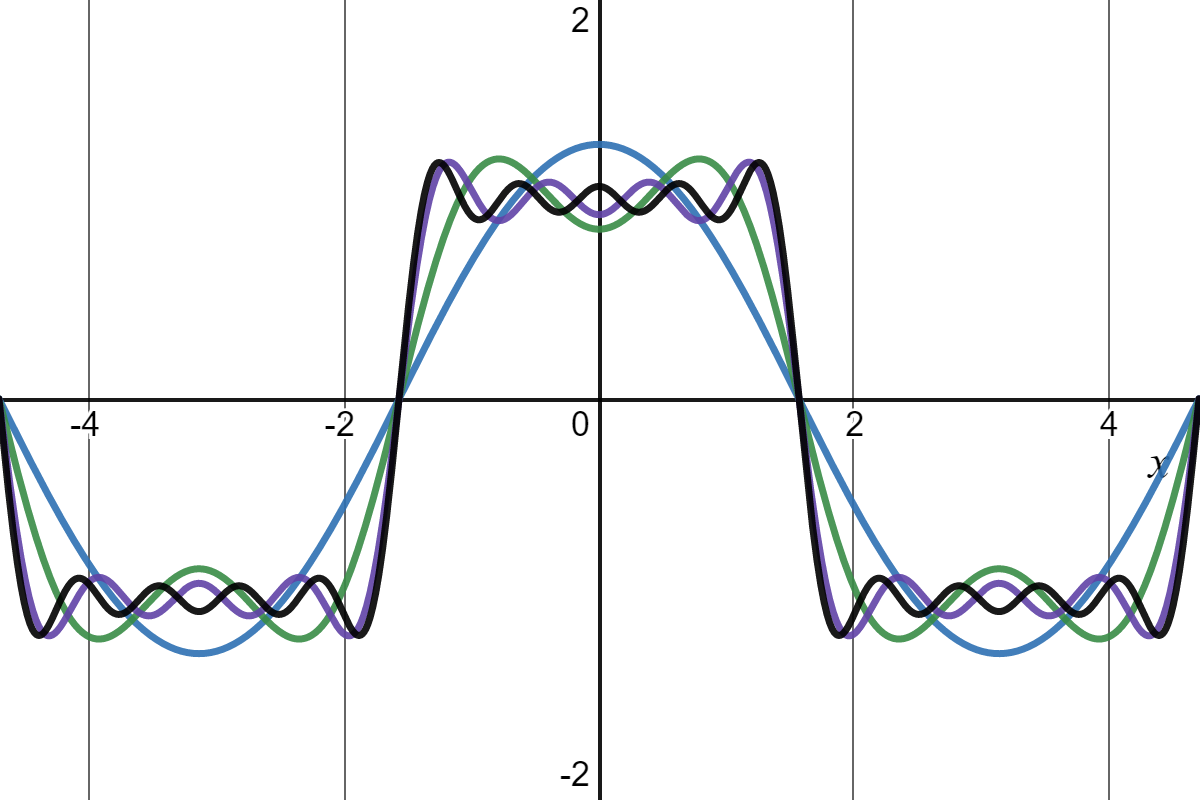
\includegraphics[width=.6\textwidth]{figures/fourier_square.png}
\end{figure}
\vfill
\end{frame}

\begin{frame}{Fourier series}
\vfill
\begin{itemize}
    \pause
    \item He then uses this solution to show the general solution to the heat equation for two rods of different constant temperatures that come into contact at time $t=0$.
    \pause
    \item Ultimately, he determines that one can determine coefficients in the series
    \[
    f(x) = c_0 + \sum_{n=1}^\infty a_n \cos(nx) + \sum_{n=1}^\infty b_n \sin(nx)
    \]
 via integrals 
    \[
    a_n = \frac{2}{\pi}\int_{-\pi/2}^{\pi/2} f(x) \cos(nx)dx \qquad     b_n = \frac{2}{\pi}\int_{-\pi/2}^{\pi/2} f(x) \sin(nx)dx.
    \]
\end{itemize}
\vfill
\end{frame}

\section{Reception}

\begin{frame}{}
    \vfill
    \begin{itemize}
    \pause
    \item This treatise, finished in 1807, was not well received by his advisors Laplace and Lagrange.
    \pause
    \item They did not really believe his work and told him not to publish.
    \pause
    \item Biot and Poisson both attacked the theory as well. Fourier proved Biot's alternate route false. Poisson claimed to have another theory.
    \pause
    \item Fourier eventually published in 1822.
\end{itemize}
    \vfill
\end{frame}

\begin{frame}{}
\vfill
\begin{center} \Large{And the rest is history...} \end{center}
\vfill
\end{frame}





\end{document}